


Introduction

Finance itself is a relatively young field of research in which data have been available in large quantities only over the last 20 years. Thanks to electronic trading, it is now possible to quantify and analyze the fluctuations of financial markets on a large scale, but much interdisciplinary expertise is necessary to make headway in understanding it all.
Examples of Statistics and Probability
getstats campaign
Florence Nightingale
AdHoc Fallacy
Post Hoc Ergo Propter Hoc
Ecological Fallacy
2004 Washington State Gubernatorial Election

Shewhart Control Charts
Deming

Cluster Sampling

Quota Sampling
Variables

Variables are things that we measure, control, or manipulate in research.


Sample size.
For this course the sample size is always denoted n.
Measures of Centrality
The mean 

The mean (sometimes pronounced "x-bar") is the most commonly used measure of centrality.

The Median


s2=i=1n(xi-x)2n-1
The Normal Distribution
Use of the Standard Normal Distribution in Finance

Nicholas Nassim Taleb, author of the "Black Swan" and “Fooled by Randomness” has cautioned against the use of the normal distributions in finance.

A Fat Tail
A fat tailed probability distribution is one in which extreme events are more probable.

For example the normal distribution is typically a very good fit over a wide range of the most likely outcomes in finance. However, it is generally accepted that extreme events such as crashes are more probable it suggests.

This means that a model based on the normal distribution will give good estimates over a reasonable range, but still under-estimate extremes. For example a model might accurately estimate the chance of a share price falling 10%, but greatly under-estimate the chance of the market falling 50%.

Although there is no great difficulty in producing fat tailed probability distributions, actually producing useful valuation or risk models with these is more difficult.

A great advantage of the normal distribution is that it is mathematically easy to handle. Assuming it makes it possible to derive formulae such as Black-Scholes. Using a fat-tailed distribution would make deriving a formula more difficult or impossible. It is sometimes possible to avoid the need for formulae by modelling using a computational approach such as a Monte-Carlo simulation.



Wild Randomness

What is wild randomness? Simply put, it is an environment in which a single observation or a particular number can impact the total in a disproportionate way. The bell curve has “thin tails” in the sense that large events are considered possible but far too rare to be consequential. 

But many fundamental quantities follow distributions that have “fat tails” – namely, a higher probability of extreme values that can have a significant impact on the total.

Ignorance probably played the larger role, he thinks. Rating agencies, like investors and regulators, rely on relatively simple models to forecast the risk associated with future market movements. Those models often assume a "mild randomness" of market fluctuations. 

In reality, Cont argues, what visionary mathematician Benoît Mandelbrot calls "wild randomness" prevails: Risk is concentrated in a few rare, hard-to-predict, but extreme, market events.
The Central Limit Theorem




The Chi-Square Test
 
Categorical data
 
The Chi –Square test for independence
 
Simple Linear regression
y is the predicted value for y 


Estimate for the intercept

Estimate for the slope

The residual
The residual is the difference of the predicted value and the observed value for each case i.

case
x
y
y
Residual



Simpson's paradox




\chapter{Stochastic Processes}

\section{Probability}

Probability generating function

\begin{equation}
G_N(s) = \sum_{n=0}^{\infty} p_{n}s^{n}
\end{equation}

\begin{equation}
\frac{dG(s)}{ds} = G^{\prime}(s) = \sum_{n=1}^{\infty}
np_{n}s^{n-1}
\end{equation}


\begin{equation}
\frac{d^2G(s)}{ds^2} = G^{\prime \prime}(s) =
\sum_{n=2}^{\infty}n(n-1)p_{n}s^{n-2}
\end{equation}

\begin{equation}
G_N(1) = \sum_{n=0}^{\infty} p_{n}
\end{equation}

\begin{equation}
G^{\prime}_N(1) = \sum_{n=1}^{\infty} np_{n}=E(N) = \mu
\end{equation}


The random variable N has a binomial distribution with paramtrics
terms m and p. Its probability function is given by
\begin{equation}
p(n) = p_n  = P(N=n) = {m \choose n}p^nq^{m-n}
\end{equation}

Find its probability generating function.

\begin{equation}
G(s) =  \sum_{n=0}^{m} s^n {m \choose n} p^nq^{m-n}
\end{equation}

\begin{equation}
G(s) =  \sum_{n=0}^{m} {m \choose n} (ps)^n q^{m-n}
\end{equation}


\begin{equation}
G(s) =  (q + ps)^m
\end{equation}


\[
(x + y)^k = [{k \choose 0}x^{k}y^{0}] + [{k \choose
	1}x^{k-1}y^{1}] +  \dots + [{k \choose n}x^{k-n}y^{n}] + \dots [{k
	\choose k-1}x^{1}y^{k-1}] + [ {k \choose k}x^{0}y^{k}]
\]

\[
(x + y)^k = \sum_{n=0}^{k} {k \choose n}x^{k-n}y^{n}
\]

\[
(x + y)^3 = \left[{3 \choose 0}x^{3-0}y^{0}\right] + \left[{3
	\choose 1}x^{3-1}y^{1}\right] +  \left[ {3 \choose
	2}x^{3-2}y^{2}\right] + \left[ {3 \choose 3}x^{3-3}y^{3}\right]
\]

\[
(x + y)^3 = x^{3} + 3x^2y + 3xy^2 + y^{3}
\]


\[
\sum_{n=0}^{k} {k \choose n}p^{k-n}q^{n} = (p + q)^k
\]
This result is not interesting because $p+q=1$

\[
(p + q)^k = 1^{k} = 1
\]
However when using terms $ps$ and $q$ we can say:
\[
\sum_{n=0}^{k} {k \choose n}ps^{k-n}q^{n} = (ps + q)^k
\]


\[
{m \choose n}  = \frac{m!}{n! \times (m-n)!} \]

\section{Poisson}

\[ p(x) = \frac{e^{\alpha}\alpha^{x}}{x!} \qquad x = 0, 1,2 \dots
\]

variance and mean are both equal to $\alpha$.

\section{PGF}

\[
G(s) = \frac{1-\alpha(1-s)}{1+\alpha(1+s)}
\]












\chapter{ANOVA and Experimental Design }

\section{Designed Experiments}
\begin{itemize}
	\item In observational studies you try to examine and measure things as they naturally occur. In experimental studies you impose some manipulation and measure its effects. It is easier to generalize from
	observational studies, but it is easier to determine causality from experimental studies.
	\item The objects on which an experiment is performed are called the experimental units. Human experimental units used to be called subjects," but we now call them research participants."
	\item The explanatory variables in an experiment are referred to as factors, while the values each factor
	can have are called its levels. A specifoc experimental condition applied to a set of units is called a
	treatment.
	\item The effectiveness of a treatment is generally measured by comparing the results of units that underwent
	the treatment to the results of units in a control condition. Units in a control condition go through the
	experiment but never receive the treatment.
	\item It is generally not a good idea to determine the e®ect of a treatment by comparing the units before
	the treatment to the same units after the treatment. Just being in an experiment can sometimes cause
	changes, even if the treatment itself doesn't really do anything. This is called the placebo effect.
	\item The basic idea of an experiment is that if you control for everything in the environment except for
	the factor that you manipulate, then any differences you observe between different groups in your
	experiment must be caused by the factor. It is therefore very important that the groups of experimental
	units you have in each level of your factor are basically the same. If there is some difference between
	the types of units in your groups, then the results might be caused by those differences instead of your
	treatment.
	\item Sometimes people use matching to make their groups similar. In this case you assign people to the
	different levels of your factor in such a way that for every person in one factor level you have a similar
	person in each of the other levels.
	\item The preferred way to make your groups similar is by randomization. In this case you just randomly
	pick people to be in each of your groups, relying on the fact that on average the differences between
	the groups will average out. Not only does this require less effort, but you don't have to know ahead
	of time what are the important things that you need to match on.
	\item There are many different ways to randomly assign your experimental units to conditions. You can use
	a table of random numbers, a mathematical calculator that produces random digits, or you can use
	statistical software.
	\item Randomization is one of the basic ideas behind statistics. When we randomly assign units to be in
	either the treatment or control conditions, there will be some differences between the groups. However,
	this is not a problem because mathematicians know a lot about how random variables work. When we
	see a difference between the groups we can figure out the probability that the difference is just due to
	the way that we assigned the units to the groups. If the probability is too low for us to believe that the
	results were just due to chance we say that the difference is statistically significant, and we conclude
	that our treatment had an effect.
	\item In conclusion, when designing an experiment you want to:
	\begin{enumerate}
		\item Control the effects of irrelevant variables.
		\item Randomize the assignment of experimental units to treatment conditions
		\item Replicate your experiment across a number of experimental units.
	\end{enumerate}
\end{itemize}




\subsection{ $2^2$ Design}

The simplest type of $2^k$ design is the $2^2$, i.e. two factors, A nd B, each with two levels. We usually think of these levels as the low and high levels of the factor.


\section{Analysis of Two-factor Designs}

A two-factor analysis of variance consists of three significance tests: a test of each of the two main effects and a test of the interaction of the variables. An analysis of variance summary table is a convenient way to display the results of the significance tests. A summary table for the hypothetical experiment described in the section on factorial designs and a graph of the means for the experiment are shown below.

\begin{verbatim}
Sum of        Mean
SOURCE   df      Squares      Square      F       p
T    1    47125.3333  47125.3333  384.174   0.000
D    2       42.6667     21.3333    0.174   0.841
TD    2     1418.6667    709.3333    5.783   0.006
ERROR   42     5152.0000    122.6667
TOTAL   47    53738.6667
\end{verbatim}

\subsection{Sources of Variation}

The summary table shows four sources of variation: (1) Task, (2) Drug dosage, (3) the Task x Drug dosage interaction, and (4) Error.

\subsection{Degrees of Freedom}

\begin{itemize}
	\item The degrees of freedom total is always equal to the total number of numbers in the analysis minus one. The experiment on task and drug dosage had eight subjects in each of the six groups resulting in a total of 48 subjects. Therefore, df total = 48 - 1 = 47.
	
	\item The degrees of freedom for the main effect of a factor is always equal to the number of levels of the factor minus one. Therefore, df task = 2 - 1 = 1 since there were two levels of task (simple and complex). Similarly, df dosage = 3 - 1 = 2 since there were three levels of drug dosage (0 mg, 100 mg, and 200 mg).
	
	\item The degrees of freedom for an interaction is equal to the product of the degrees of freedom of the variables in the interaction. Thus, the degrees of freedom for the Task x Dosage interaction is the product of the degrees of freedom for task (1) and the degrees of freedom for dosage (2). Therefore, df Task x Dosage = 1 x 2 = 2.
	
	\item The degrees of freedom error is equal to the degrees of freedom total minus the degrees of freedom for all the effects. Therefore, df error = 47 - 1 - 2 - 2 = 42.
\end{itemize}

\subsection{Mean Squares}
As in the case of a one-factor design, each mean square is equal to the sum of squares divided by the degrees of freedom. For instance, Mean square dosage = 42.6667/2 = 21.333 where the sum of squares dosage is 42.6667 and the degrees of freedom dosage is 2.


\subsection{F Ratios}
The F ratio for an effect is computed by dividing the mean square for the effect by the mean square error. For example, the F ratio for the Task x Dosage interaction is computed by dividing the mean square for the interaction ( 709.3333) by the mean square error (122.6667). The resulting F ratio is: F = 709.3333/122.6667 = 5.783


\subsection{Probability Values}
To compute a probability value for an F ratio, you must know the degrees of freedom for the F ratio. The degrees of freedom numerator is equal to the degrees of freedom for the effect. The degrees of freedom denominator is equal to the degrees of freedom error. Therefore, the degrees of freedom for the F ratio for the main effect of task are 1 and 42, the degrees of freedom for the F ratio for the main effect of drug dosage are 2 and 42, and the degrees of freedom for the F for the Task x Dosage interaction are 2 and 42.

An F distribution calculator can be used to find the probability values. For the interaction, the probability value associated with an F of 5.783 with 2 and 42 df is 0.006.

\subsection{Drawing Conclusions}

When a main effect is significant, the null hypothesis that there is no main effect in the population can be rejected. In this example, the effect of task was significant. Therefore it can be concluded that, in the population, the mean time to complete the complex task is greater than the mean time to complete the simple task (hardly surprising). The effect of dosage was not significant. Therefore, there is no convincing evidence that the mean time to complete a task (in the population) is different for the three dosage levels

The significant Task x Dosage interaction indicates that the effect of dosage (in the population) differs depending on the level of task. Specifically, increasing the dosage slows down performance on the complex task and speeds up performance on the simple task. The effect of increasing the dosage therefore depends on whether the task is complex of simple.

There will always be some interaction in the sample data. The significance test of the interaction lets you know whether you can infer that there is an interaction in the population.



%--------------------------------------------------------------------------------------------------%
\section{Fractional factorial design}

(d)	Define the following terms used in fractional factorial design; Defining relation,
Generator, Confounding, Resolution. Which design resolution is considered
optimal?
\section{Factorial Design}
Factorial experiments permit researchers to study behavior under conditions in which independent variables, called in this context factors, are varied simultaneously.

Thus, researchers can investigate the joint effect of two or more factors on a dependent variable. The factorial design also facilitates the study of interactions, illuminating the effects of different conditions of the experiment on the identifiable subgroups of subjects participating in the experiment.


A full factorial experiment is an experiment whose design consists of two or more factors, each with discrete possible values or ``levels", and whose experimental units take on all possible combinations of these levels across all such factors. A full factorial design may also be called a fully-crossed design. Such an experiment allows studying the effect of each factor on the response variable, as well as the effects of interactions between factors on the response variable.

For the vast majority of factorial experiments, each factor has only two levels. For example, with two factors each taking two levels, a factorial experiment would have four treatment combinations in total, and is usually called a $2\times2$ factorial design.

\newpage

\section{Completely Randomized Design}

\subsection{Questions}
\begin{itemize}
	\item Give the principal features of a  balanced completely randomised design, and
	explain the role of replication in such a design.  \item State the statistical model for
	this design, define the terms in the model and state the standard assumptions
	made about the error term.
	\item Briefly explain the principles of randomisation and replication, in the
	context of a completely randomised experimental design. Write down the model equation for a completely randomised design
	having equal numbers of replicates in all treatment groups, defining all
	the symbols that you use.
\end{itemize}
%--------------------------------------------------------%
\section{Orthogonal Array}
Orthogonal array testing is a systematic, statistical way of testing. Orthogonal arrays can be applied in user interface testing, system testing, regression testing, configuration testing and performance testing.
All orthogonal vectors exhibit orthogonality. Orthogonal vectors exhibit the following properties:
Each of the vectors conveys information different from that of any other vector in the sequence, i.e., each vector conveys unique information therefore avoiding redundancy.
On a linear addition, the signals may be separated easily.
Each of the vectors is statistically independent of the others.
When linearly added, the resultant is the arithmetic sum of the individual components.


\subsection{Two Factor Interaction}
The effects of interest in the $2^2$ design are the  main effects A and B and the two-factor interaction AB. It is easy to estimate the effects of these factors.

\begin{eqnarray}
A = \frac{a+ab}{2n} -  \frac{b + (1)}{2n}\\
B = \frac{b+ab}{2n} -  \frac{a + (1)}{2n}\\
AB = \frac{ab + (1)}{2n} -  \frac{a + b}{2n}\\
\end{eqnarray}

The Sums of Squares formulae are
\begin{eqnarray}
SS_{A} = \frac{[(a + ab)-(b + (1))]^2}{4n^2}\\
SS_{B} = \frac{[(b + ab)-(a + (1))]^2}{4n^2}\\
SS_{AB} = \frac{[(ab + (1))-(a + b)]^2}{4n^2}\\
\end{eqnarray}

%---------------------------------------------------------------------%
%---------------------------------------------------------------------%
%---------------------------------------------------------------------%






\chapter{Reliability Theory}

\section{Notation}\begin{enumerate}
	\item
	F(t) : Failure function. Probability that a component fails
	before time `t'.
	\item R(t) : Reliability function ( Survivor function) Probability that a component
	has survived to time `t'.
	\item r(t) : Failure rate function (hazard function)
\end{enumerate}

\section{Reliability Theory}

\begin{enumerate}
	\item Exponential distribution and reliability\item Mean time to
	failure \item Reliability of series and parrallel systems \item
	Renewal processes\end{enumerate}
\newpage
\chapter{Introduction to \texttt{R}}

\section{The \texttt{R} Project for Statistical Computing}

\texttt{R} is a language and environment for statistical computing and graphics. \texttt{R}provides a wide variety of statistical and graphical techniques, and is highly extensible. Among its tools
one can find implemented
\begin{itemize}
	\item linear and nonlinear modelling,
	\item classical statistical tests,
	\item time-series analysis,
	\item classification,
	\item clustering,
	\item ...and many more.
\end{itemize}
One of R's strengths is the ease with which well-designed publication quality plots can be produced.
including mathematical symbols and formulae where needed.
\begin{itemize} \item
	\texttt{R} is a computing software for statistical analysis \item The package is available for all popular operating systems: Windows, Mac or Linux.
	\item It is free!
	\item Everyone (knowledgeable enough) can contribute to the software by
	writing a package.
	\item Packages are available for download through a convenient facility
	\item It is fairly well documented and the documentation is available either
	from the program help menu or from the web-site.
	\item It is the top choice of statistical software among academic statisticians
	but also very popular in industry specially among biostatisticians and
	medical researchers (mostly due to the huge package called
	Bioconductor that is built on the top of \texttt{R}).
	\item It is a powerful tool not only for doing statistics but also all kind of
	scientific programming.
\end{itemize}


\texttt{R} is an integrated suite of software facilities for data manipulation, calculation and graphical display. It
includes
\begin{itemize}
	\item an effective data handling and storage facility,
	\item a suite of operators for calculations on arrays, in particular matrices,
	\item a large, coherent. integrated collection of intermediate tools for data analysis,
	graphical facilities for data analysis and display either on-screen or on hard-copy, and
	\item a well-developed, simple and effective programming language which includes conditionals, loops,
	user-defined recursive functions and input and output facilities.
\end{itemize}

\section{Downloading and Installing \texttt{R}}

\begin{itemize}
	\item \texttt{R} can be downloaded from the CRAN website: http://cran.r-project.org/
	\item You may choose versions for windows, mac and linux.
	\item As per the instructions on the respective pages, you require the ``base" distribution.
	\item Now you can download the installer for latest version of \texttt{R} , version 2.17.
	\item Select the default settings. Once you finish, the \texttt{R} icon should appear on your desktop.
	\item Clicking on this icon will start up the program.
\end{itemize}

\section{Statistical Tables using \texttt{R}}
The following is a fragment of the tables of the values of $F(x)$ for the standard normal (`Z') cumulative distribution function from page 254 of the main textbook.
% Reproduction of Tables

%\begin{center}
%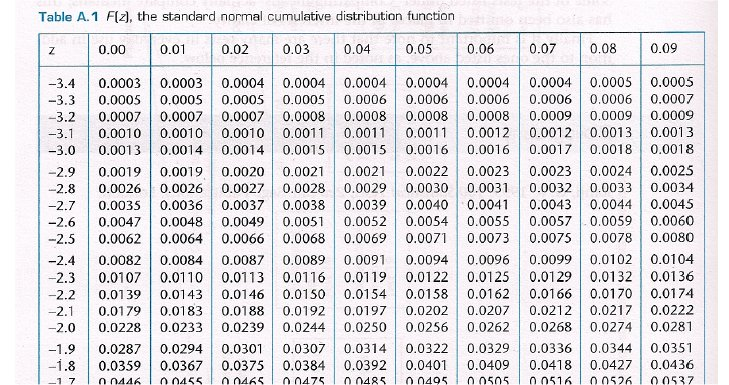
\includegraphics[scale=0.6]{Image6}
%\end{center}
\newpage
\begin{center}
	\line(1,0){250}
\end{center}

\begin{verbatim}
# Segment 1A-1
# Preceding line with the symbol ’#’ makes it a comment in R
# The following line produce a single value of the standard normal cumulative
# function. It is the value corresponding to the first value in the table

pnorm(-3.4)

#[1] 0.0003369293
#Then the first row of the table

z=seq(-3.4,-3.31,by=0.01)
pnorm(z)

# [1] 0.0003369293 0.0003494631 0.0003624291 0.0003758409 0.0003897124
# [6] 0.0004040578 0.0004188919 0.0004342299 0.0004500872 0.0004664799
# And all values from the table

z=seq(-3.4,3.4,by=0.01)
pnorm(z)

#  [1] 0.0003369293 0.0003494631 0.0003624291 0.0003758409 0.0003897124
#  [6] 0.0004040578 0.0004188919 0.0004342299 0.0004500872 0.0004664799
# [11] 0.0004834241 0.0005009369 0.0005190354 0.0005377374 0.0005570611
# [16] 0.0005770250 0.0005976485 0.0006189511 0.0006409530 0.0006636749
# [21] 0.0006871379 0.0007113640 0.0007363753 0.0007621947 0.0007888457
# [26] 0.0008163523 0.0008447392 0.0008740315 0.0009042552 0.0009354367
# [31] 0.0009676032 0.0010007825 0.0010350030 0.0010702939 0.0011066850

\end{verbatim}
\begin{center}
	\line(1,0){250}
\end{center}
\newpage
There is more than meets the eye in the table. It is not only the table values that can be explored for the
standard normal distribution using \texttt{R}. Recall that the normal
distribution is defined by the density function:
\[
f(z) = \frac{1}{\sqrt(2 \pi)}e^{-Z^2/2}.
\]

The density represents distribution of probability for a random variable associated with it.
The area under the density represents the probability so the that the total area under it is equal to one.
The area accumulated up to certain value $z_o$ represents probability that a corresponding random variable takes
value smaller than z and this probability defines the cumulative distribution function $F(z)$ which is tabularized.


All this can be seen in \texttt{R}. The following code explores various aspects of the standard normal distribution:
\begin{center}
	\line(1,0){250}
\end{center}
\begin{verbatim}

#Plotting the density function of the standard normal variable
z=seq(-3,3,by=0.01)
plot(z,dnorm(z),type='l',col="red",lwd=4)

#Plotting the cumulative distribution function (that one from the table)
plot(z,pnorm(z),type='l',col="red",lwd=4)

\end{verbatim}
\begin{center}
	\line(1,0){250}
\end{center}
\newpage
The \texttt{R} code results in the following plots.
\begin{itemize}
	\item The probability density function.
	\item The cumulative density function.
\end{itemize}
\begin{center}
	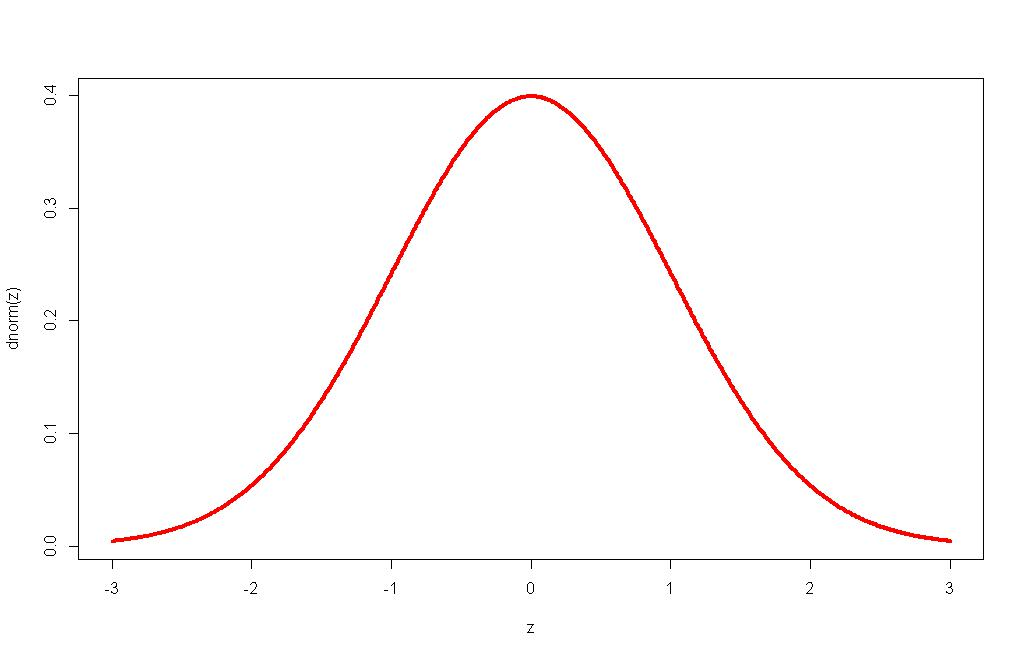
\includegraphics[scale=0.3]{Image7a}
\end{center}
\begin{center}
	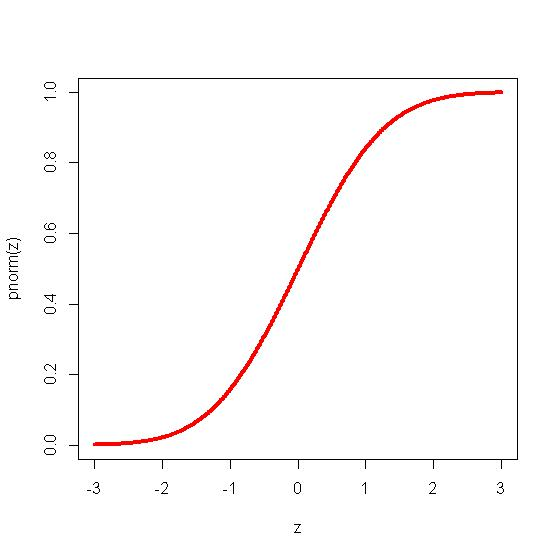
\includegraphics[scale=0.5]{Image7b}
\end{center}
\newpage

\section{Data Analysis with \texttt{R}}

Data from Table 1.1 of the textbook

Table 1.1 Random and systematic errors

\begin{tabular}{|c|ccccc|l|}
	\hline
	% after \\: \hline or \cline{col1-col2} \cline{col3-col4} ...
	Student & Results  & (ml) &  &  &  &Comment \\ \hline
	A & 10.08 & 10.11 &10.09 &10.10&10.12 & Precise, unbiased\\ \hline
	B & 9.88 &10.14& 10.02 &9.80& 10.21& Imprecise unbiased\\ \hline
	C & 10.19 &9.79& 9.69 &10.05& 9.78 & Imprecise, biased\\ \hline
	D & 10.04 &9.98 &10.02 &9.97 &10.04 & Precise, unbiased \\
	\hline
\end{tabular}
\bigskip

This is also given in the text file Table$1-1$.txt, the contents of which is given below:
\begin{center}
	\line(1,0){250}
\end{center}
\begin{verbatim}
A 10.08 10.11 10.09 10.10
B 9.88 10.14 10.02 9.80
C 10.19 9.79 9.69 10.05
D 10.04 9.98 10.02 9.97
\end{verbatim}
\begin{center}
	\line(1,0){250}
\end{center}

Reading data from a file to \texttt{R}:
\begin{center}
	\line(1,0){250}
\end{center}
\begin{verbatim}
#Reading the data from
Titra=read.table("Table1-1.txt", row.names = 1)
Titra
# V2 V3 V4 V5
#A 10.08 10.11 10.09 10.10
#B 9.88 10.14 10.02 9.80
#C 10.19 9.79 9.69 10.05
#D 10.04 9.98 10.02 9.97
#Listing the first row
Titra[1,]
#and the fourth column
Titra[,4]
\end{verbatim}
\begin{center}
	\line(1,0){250}
\end{center}

\textbf{Means and standard deviations}\\

Find the mean and standard deviation of A's results.

\begin{center}
	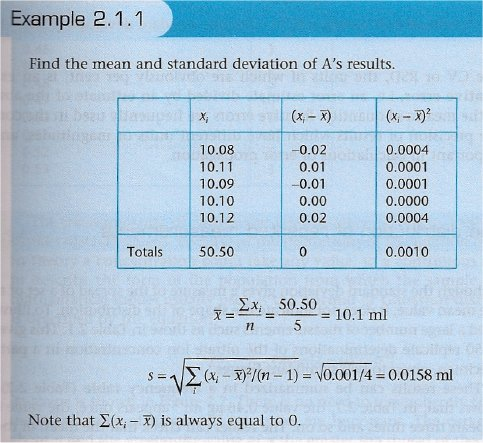
\includegraphics[scale=0.6]{Image8}
\end{center}


\textbf{Means and standard deviations much faster and better}
\begin{center}
	\line(1,0){250}
\end{center}
\begin{verbatim}
#Comuting means
rowMeans(Titra)
# A B C D
#10.0950 9.9600 9.9300 10.0025
#and standard deviation
apply(Titra,1,sd)
# A B C D
#0.01290994 0.15055453 0.23036203 0.03304038
\end{verbatim}
\begin{center}
	\line(1,0){250}
\end{center}
\newpage
\textbf{Nitrate ion concentration from Table 2.1}\\
Table 2.1 Results of 50 determinations of nitrate ion concentration, in $\mu$g $ml^{-1}$ (Also in the file Table $2-1$.txt.) \\
\begin{tabular}{|c|c|c|c|c|c|c|c|c|c|}
	\hline
	0.51 &0.51 &0.51 &0.50 &0.51 &0.49 &0.52 &0.53 &0.50 &0.47\\
	0.51 &0.52 &0.53 &0.48 &0.49 &0.50 &0.52 &0.49 &0.49 &0.50\\
	0.49 &0.48 &0.46 &0.49 &0.49 &0.48 &0.49 &0.49 &0.51 &0.47\\
	0.51 &0.51 &0.51 &0.48 &0.50 &0.47 &0.50 &0.51 &0.49 &0.48\\
	0.51 &0.50 &0.50 &0.53 &0.52 &0.51 &0.50 &0.50 &0.51 &0.51\\
	\hline
\end{tabular}\\ \bigskip

\begin{center}
	\line(1,0){250}
\end{center}
\begin{verbatim}
0.51 0.51 0.51 0.50 0.51 0.49 0.52 0.53 0.50 0.47
0.51 0.52 0.53 0.48 0.49 0.50 0.52 0.49 0.49 0.50
0.49 0.48 0.46 0.49 0.49 0.48 0.49 0.49 0.51 0.47
0.51 0.51 0.51 0.48 0.50 0.47 0.50 0.51 0.49 0.48
0.51 0.50 0.50 0.53 0.52 0.51 0.50 0.50 0.51 0.51
\end{verbatim}
\begin{center}
	\line(1,0){250}
\end{center}
Compute the mean concentration, and the standard deviation:
\begin{center}
	\line(1,0){250}
\end{center}
\begin{verbatim}
#Getting data in a vector
x=scan('Table2_1.txt')
mean(x)
#[1] 0.4998
sd(x)
#[1] 0.01647385
\end{verbatim}
\begin{center}
	\line(1,0){250}
\end{center}
\newpage

\subsection{Bootstrap Methods}
If we would repeat our experiment of collecting 50 samples of nitrate concentrations many times we would see the range of error. But it would be a waste of resources and not a viable method.\\
Instead we re-sample `new' data from our data and use so obtained new samples for assessment of the error.
The following \texttt{R} code does the job.
\begin{center}
	\line(1,0){250}
\end{center}
\begin{verbatim}
#Getting data in a vector
m=mean(x)
bootstrap=vector('numeric',500)
for(i in 1:500)
{
bootstrap[i]=mean(sample(x,replace=T))-mean(x)
}
#The distribution of estimation error
hist(bootstrap)
\end{verbatim}
\begin{center}
	\line(1,0){250}
\end{center}
The conclusion of this procedure is that the nitrate concentration is $4999 \pm 0.005$. We are specifically interested in how \texttt{R} was easily able to implement a solution for this.
\newpage
\section{Introduction - systematic vs. random errors}




\section{Statistics of Repeated Measures}
\subsection{Titration experiment}

Recall the titration experiment from the last class. 4 Students performing the same experiment five times, hence each yield 5 results.(Table 1.1 random and systematic errors).


\begin{tabular}{|c|ccccc|l|}
	\hline
	% after \\: \hline or \cline{col1-col2} \cline{col3-col4} ...
	Student & Results  & (ml) &  &  &  &Comment \\ \hline
	A & 10.08 & 10.11 &10.09 &10.10&10.12 & Precise, biased\\ \hline
	B & 9.88 &10.14& 10.02 &9.80& 10.21& Imprecise unbiased\\ \hline
	C & 10.19 &9.79& 9.69 &10.05& 9.78 & Imprecise, biased\\ \hline
	D & 10.04 &9.98 &10.02 &9.97 &10.04 & Precise, unbiased \\
	\hline
\end{tabular}\\




Two criteria were used to compare these results, the average value (technically know
as a measure of location and the degree of spread (or dispersion). The average value
used was the arithmetic mean (usually abbreviated to \emph{the mean}), which is the sum
of all the measurements divided by the number of measurements.


The mean,$\bar{X}$, of $n$ measurements is given by \[ \bar{X}  = {\sum{x} \over n} \]

In Chapter 1 the spread was measured by the difference between the highest and
lowest values (i.e. the range). A more useful measure, which utilizes all the values, is the sample
standard deviation, $s$, which is defined as follows:

The standard deviation, $s$, of $n$ measurements is given by
\[s=  \sqrt{ {\sum(x-\bar{X})^2 \over n-1} }  (2.2) \]









Example 1
A fair die is thrown. The number shown on the die is the random variable X. Tabulate the possible outcomes.
Solution
X takes the six possible outcomes 1, 2, 3, 4, 5, 6 which each have probability 1/6 (i.e. one sixth).

r 	1 	2 	3 	4 	5 	6
P(X = r)	1/6 	1/6 	1/6 	1/6 	1/6 	1/6
Example 2
Two unbiased spinners, one numbered 1, 3, 5, 7 and the other numbered 1, 2, 3 are spun. The random variable X is the sum of the two results.
Find the probability distribution for X.



Solution
Listing all the possible outcomes is best done in a table.








%
%http://www.me.mtu.edu/~jwsuther/doe2005/notes/orth_arrays.pdf
%
%http://www.weibull.com/DOEWeb/taguchis_orthogonal_arrays.htm
%
%http://controls.engin.umich.edu/wiki/index.php/Design_of_experiments_via_taguchi_methods:_orthogonal_arrays
%
%http://elsmar.com/Taguchi.html

\newpage
\chapter{Statistics for Chemists}

\section{Quantitative nature of analytical chemistry}
Modern analytical chemistry is overwhelmingly a quantitative science.
A quantitative answer is much more valuable than a qualitative one.
It may be useful for an analyst to claim to have detected some boron in a
distilled water sample, but it is much more useful to be able to say how
much boron is present.

Often it is only a quantitative result that has any value at all.For
example, almost all samples of (human) blood serum contain albumin;
the only question is, how much ? Even where a qualitative answer is required, quantitative methods are
used to obtain it.

Quantitative approaches might be used to compare two soil samples. For example, they might be subjected to a particle
size analysis, in which the proportions of the soil particles falling within a number say 10, of particle-size ranges are determined. Each sample would then be characterized by these 10 pieces of data, which could
then be used to provide a quantitative assessment of their similarity.

\subsection{Errors in quantitative analysis}
Since quantitative studies play a dominant role in any analytical laboratory, it must be accepted that the errors that occur in such studies are of supreme importance. No quantitative results are of any value unless they are accompanied by some estimate of the errors inherent in them!
\newpage
\noindent \textbf{Example 1 - detecting a new analytical reagent}\\
\begin{itemize} \item A chemist synthesizes an analytical reagent that is believed to be entirely new.
	\item The compound is studied using a spectrometric method and gives a
	value of 104.
	\item The chemist finds that no compound previously discovered has yielded
	a value of more than 100.
	\item Has the chemist really discovered a new compound?
	\item The answer lies in the degree of reliance to experimental value of 104.
	\item If the result is correct to within 2 (arbitrary) units, i.e. the true value
	probably lies in the range $102\pm 2$, then a new material has probably
	been discovered.
	\item If, however, investigations show that the error may amount to 10 units
	i.e. $104 \pm 10$, then it is quite likely that the true value is actually less than
	100, in which case a new discovery is tar from certain.
	\item A knowledge of the experimental errors is crucial!!
\end{itemize}

\newpage
\textbf{Example 2 - replicates in a titrimetric experiment}\\
\begin{itemize}
	\item Analysts commonly perform several replicate determinations in the
	course of a single experiment.
	\item An analyst performs a titrimetric experiment four times and obtains
	values of 24.69,24.73,24.77 and 25.39 ml.
	\item All four values are different, because of the variations inherent in the
	measurements
	\item The fourth value (25.39 ml) is substantially different from the other three.
	\item Can it be safely rejected, so that (for example) the mean titre is reported
	as 24.73 ml, the average of the other three readings?
\end{itemize}

\section{Comapring Methods of Measurement}

\subsection{The Bland Altman plot}
The Bland Altman plot (Bland \& Altman, 1986 and 1999) is a statistical method to compare two measurements techniques. In this graphical method the differences (or alternatively the ratios) between the two techniques are plotted against the averages of the two techniques. Horizontal lines are drawn at the mean difference, and at the limits of agreement, which are defined as the mean difference plus and minus 1.96 times the standard deviation of the differences.

\chapter{Chemometrics}

\section{Chemometrics}

\begin{enumerate}
	\item Calibration \item Paired T test \item Confidence intervals
\end{enumerate}


\section{Calibration}

\section{Blank Signals}
\newpage
\section{Chemometrics}
\begin{itemize}
	\item  Chemometrics is the science of extracting information from chemical systems by statistical means.
	\item An analyte is a substance or chemical constituent that is determined in an analytical procedure, such as a titration.
	\item the detection limit, lower limit of detection, or LOD (limit of detection), is the lowest quantity of a substance that can be distinguished from the absence of that substance (a blank value) within a stated confidence limit (generally 1\%).
	\item The detection limit is estimated from the mean of the blank, the standard deviation of the blank and some confidence factor. Another consideration that affects the detection limit is the accuracy of the model used to predict concentration from the raw analytical signal.
	
\end{itemize}

\subsection{Geometric notation}

%------------------------------------------------------------------------------------------------%
\chapter{ Information Theory and Data Compression}

\section{Data Compression}
\begin{itemize}
	\item[1.] Explain what an optimal code is, in the context of data compression.
	\item[2.] Are Huffman Codes Optimal?
\end{itemize}


The frequency of 0 as an input to a binary channel is 0.6. If O is the
input, then 0 is the output with probability 0.8. If l is the input, then l
is the output with probability 0.9.
\begin{itemize}
	\item[a.](4 marks) Calculate the information per bit contained in the input.
	\item[b.](2 marks)Calculate the probability that the output is 0.
	\item[c.](2 marks) Calculate the probability that the output is l,
	\item[d.](2 marks) Calculate the probability that the input is 0 given that the
	output is O.
	\item[e.](2 marks) Calculate the probability that the input is l given that
	the output is 1,
	\item[f.](2 marks) Calculate the probability that the input is l given that
	the output is O.
	\item[g.](2 marks) Calculate the probability that the input is 0 given that
	the output is l.
	\item[h.](6 marks) Calculate the amount of information transmitted by the channel.
	\item[i.](3 marks) Derive the globally optimal reconstruction rule.
\end{itemize}




\subsection*{Information Theory}

\begin{itemize}
	\item $I(p) = - log_{2}(p) = log_{2}(1/p)$\\
	
	\item $I(pq) = I(p) + I(q)$\\
	
	\item $H = - \sum_{i=1}^{m}p_{i}\; log_{2}(p_{i})$\\
	
	\item $E(L) = \sum_{i=1}^{m} l_{i} p_{i}$\\
	
	\item $\mbox{Efficiency} = H / E(L)$\\
	
	\item $I(X;Y) = H(X) + H(Y) - H(X,Y)$\\
	
	\item $I(X;Y) = H(X) - H(X|Y)$\\
	
	\item $P(C[r]) = \sum_{j=1}^{m}P(C[r]|Y=d_{j} )P(Y=d_{j} )$
	
\end{itemize}







\bigskip
An inspector of computer parts selects a random sample of components
from a large batch to decide whether or not to audit the full batch.
(i) If 20$\%$ or more of the sample is defective, the entire batch is
inspected, Calculate the probability of this happening if it is
thought that the population contains 4$\%$ defective components and
a sample of 20 is selected.
(ii) If 10$\%$ or more of the sample is defective, the entire batch is
inspected. Calculate the probability of this happening if it is
thought that the population contains 4$\%$ defective components and
a sample of 50 is selected.
(10 marks)
(d) A model of an on—line computer system gives a mean time to retrieve a
record from a direct access storage system device of 200 milliseconds
with a standard deviation of 58 milliseconds. If it can be assumed that
the data are normally distributed:
(i) What proportion of retrieval times will be greater than 75
milliseconds?
(ii) What proportion of retrieval times will be between 150
milliseconds and 250 milliseconds?
(iii) What is the retrieval time below which 10\% of retrieval times
will be?
(9 marks)


\begin{eqnarray*}
	r&=&\frac{S_{XY}}{\sqrt{S^2_X}\times\sqrt{S^2_Y}}.\\\\
	S_{XY}&=&\sum xy-\frac{\sum x \times \sum y}{n}.\\\\ S^2_X&=&\sum x^2-\frac{(\sum x)^2 }{n}.\\\\ S^2_Y&=&\sum y^2-\frac{(\sum y)^2 }{n}.\\\\ \end{eqnarray*} {\bf Regression coefficients} \begin{eqnarray*} \hat{\beta}_1&=&\frac{S_{XY}}{S^2_X}.\\\\
	\hat{\beta}_0&=&\bar{y}-(\hat{\beta}_1\times\bar{x}).
\end{eqnarray*}


\begin{itemize}
	\item[1.] Given four symbols A, B, C and D, the symbols occur with an equal
	probability. What is the entropy of the distribution?
	\item[2.] Suppose they occur with probabilities 0.5, 0.25, 0.125 and 0.125
	respectively. What is the entropy associated with the event (experiment)?
	\item[3.] Suppose the probabilities are 1,0,0,0. What is the entropy?
\end{itemize}

\chapter{Advanced Inference Procedures}



\section{Grubb's Test}

Grubb's Test for Detecting Outliers
Statisticians have devised several ways to detect outliers. Grubbs' test is particularly easy to follow. This method is also called the ESD method (extreme studentized deviate).
The first step is to quantify how far the outlier is from the others. Calculate the ratio Z as the difference between the outlier and the mean divided by the SD. If Z is large, the value is far from the others. Note that you calculate the mean and SD from all values, including the outlier.



Since $5\%$ of the values in a Gaussian population are more than 1.96 standard deviations from the mean, your first thought might be to conclude that the outlier comes from a different population if Z is greater than 1.96. This approach only works if you know the population mean and SD from other data. Although this is rarely the case in experimental science, it is often the case in quality control. You know the overall mean and SD from historical data, and want to know whether the latest value matches the others. This is the basis for quality control charts.

When analyzing experimental data, you don't know the SD of the population. Instead, you calculate the SD from the data. The presence of an outlier increases the calculated SD. Since the presence of an outlier increases both the numerator (difference between the value and the mean) and denominator (SD of all values), Z does not get very large. In fact, no matter how the data are distributed, Z can not get larger than, where N is the number of values. For example, if N=3, Z cannot be larger than 1.155 for any set of values.

Grubbs and others have tabulated critical values for Z which are tabulated below. The critical value increases with sample size, as expected.

If your calculated value of Z is greater than the critical value in the table, then the P value is less than 0.05. This means that there is less than a $5\%$ chance that you'd encounter an outlier so far from the others (in either direction) by chance alone, if all the data were really sampled from a single Gaussian distribution. Note that the method only works for testing the most extreme value in the sample (if in doubt, calculate Z for all values, but only calculate a P value for Grubbs' test from the largest value of Z.

Once you've identified an outlier, you may choose to exclude that value from your analyses. Or you may choose to keep the outlier, but use robust analysis techniques that do not assume that data are sampled from Gaussian populations.

If you decide to remove the outlier, you then may be tempted to run Grubbs' test again to see if there is a second outlier in your data. If you do this , you cannot use the same table.

\section{Dixon's Q test}

In statistics, Dixon's Q test, or simply the Q test, is used for identification and rejection of outliers. This test should be used sparingly and never more than once in a data set. To apply a Q test for bad data, arrange the data in order of increasing values and calculate Q as defined:

\begin{equation}
Q = \frac{\mbox{Gap}}{\mbox{Range}}
\end{equation}

Where gap is the absolute difference between the outlier in question and the closest number to it. If $Q_calculated > Q_table$, then reject the questionable point.

\section{Kolmogorov-Smirnov test}
The Kolmogorov-Smirnov test is defined by:
\\
H$_0$:     The data follow a specified distribution\\
H$_1$:     The data do not follow the specified distribution\\

Test Statistic:     The Kolmogorov-Smirnov test statistic is defined as

where F is the theoretical cumulative distribution of the distribution being tested which must be a continuous distribution (i.e., no discrete distributions such as the binomial or Poisson), and it must be fully specified

\subsection{ Characteristics and Limitations of the K-S Test}


An attractive feature of this test is that the distribution of the K-S test statistic itself does not depend on the underlying cumulative distribution function being tested. Another advantage is that it is an exact test (the chi-square goodness-of-fit test depends on an adequate sample size for the approximations to be valid). Despite these advantages, the K-S test has several important limitations:
\begin{enumerate}
	\item It only applies to continuous distributions.
	\item It tends to be more sensitive near the center of the distribution than at the tails.
	\item Perhaps the most serious limitation is that the distribution must be fully specified. That is, if location, scale, and shape parameters are estimated from the data, the critical region of the K-S test is no longer valid. It typically must be determined by simulation.
\end{enumerate}
Due to limitations 2 and 3 above, many analysts prefer to use the Anderson-Darling goodness-of-fit test.

However, the Anderson-Darling test is only available for a few specific distributions.

\section{The Anderson–Darling test}

The Anderson–Darling test is a statistical test of whether there is evidence that a given sample of data did not arise from a given probability distribution.

In its basic form, the test assumes that there are no parameters to be estimated in the distribution being tested, in which case the test and its set of critical values is distribution-free. However, the test is most often used in contexts where a family of distributions is being tested, in which case the parameters of that family need to be estimated and account must be taken of this in adjusting either the test-statistic or its critical values.

When applied to testing if a normal distribution adequately describes a set of data, it is one of the most powerful statistical tools for detecting most departures from normality.

\section{The Shapiro-Wilk test of normality}
Performs the Shapiro-Wilk test of normality.
\begin{verbatim}
> x<- rnorm(100, mean = 5, sd = 3)
> shapiro.test(x)

Shapiro-Wilk normality test

data:  rnorm(100, mean = 5, sd = 3)
W = 0.9818, p-value = 0.1834
\end{verbatim}
In this case, the p-value is greater than 0.05, so we fail to reject the null hypothesis that the
data set is normally distributed.
\begin{verbatim}
>y <- runif(100, min = 2, max = 4)
> shapiro.test(y)

Shapiro-Wilk normality test

data:  runif(100, min = 2, max = 4)
W = 0.9499, p-value = 0.0008215
\end{verbatim}
In this case, the p-value is less than 0.05, so we reject the null hypothesis that the
data set is normally distributed.



\subsection{Shapiro-Wilk test: Example}

\begin{verbatim}
> x<-rnorm(100, mean = 5, sd = 3)
> y<-runif(100, min = 2, max = 4)
> shapiro.test(x)

Shapiro-Wilk normality test
data:  x
W = 0.9851, p-value = 0.3249
>
> shapiro.test(y)
Shapiro-Wilk normality test
data:  y
W = 0.9585, p-value = 0.003151

\end{verbatim}
\newpage
%------------------------------------------------------------------------------------------------%
%------------------------------------------------------------------------------------------------%
%------------------------------------------------------------------------------------------------%
\chapter{Birth and Death Processes}


\section{Birth processes}
Generating function equations

\[
\frac{ds}{dz} = \lambda s(s-1)
\]
This is a first order separable equation.
\[
\int \frac{s(s-1)}{ds} = \int -\lambda dz = -\lambda z
\]


\section{Pure death processes}
In a pure death process, the population numbers decline by dying
off, with no replacement births.

\[ \int \frac{ds}{s(1-s)} = \int \mu dz = \mu z \]


\[ \int \frac{ds}{s(1-s)} = \int \frac{1}{s} ds 1 \int
\frac{1}{s-1}ds= ln \left[\frac{s}{1-s} \right]
\]

\[  \mbox{ln} \left[\frac{s}{1-s} \right] = -\lambda z
\]

\[  \left[\frac{s}{1-s} \right] = exp(-\lambda z)
\]

\[  s = \left[\frac{1}{1+exp(-\lambda z)} \right]
\]

\subsubsection{Calculations}
\begin{enumerate} \item  $ \frac{1}{s(1-s)} = \frac{1}{s} + \frac{1}{1-s} =
	\frac{1}{s} - \frac{1}{s-1}$
	\item $ \mbox{ln}(a-b) = \mbox{ln}(\frac{a}{b})$\\
\end{enumerate}

\section{Combined birth and death processes}
birth rate $\lambda$ and death rate $\mu$.


\newpage
\chapter{Assorted Topics}

\section{Testing Normality}

\begin{itemize}
	\item Normal probability plot \item Outliers \item dixon test
	\item Grubbs test
\end{itemize}


\section{Mallow's Cp}
Mallow's $Cp$ coefficient is a metric used in model selection to
dissuade the use of over-fitted models.

\begin{equation}
Cp= \frac{RSS}{\hat{\sigma}^{2}}-(n-2p)
\end{equation}
This coefficient should be minimized over $p$.

\begin{enumerate}
	\item Multicollinearity
	\item Biometrics
	\item Variance Inflation Factor
	\begin{enumerate}
		\item The heights for a group of forty rowing club members are tabulated as follows;
		
		\begin{table}[ht]
			\begin{center}
				\begin{tabular}{|rrrrrrrrrr|}
					
					\hline
					141 & 148 & 149 & 149 & 155 & 156 & 167 & 169 & 169 & 170 \\
					171 & 173 & 175 & 176 & 177 & 179 & 182 & 182 & 183 & 183 \\
					183 & 184 & 184 & 184 & 185 & 185 & 185 & 186 & 186 & 189 \\
					191 & 191 & 191 & 191 & 192 & 192 & 192 & 193 & 194 & 199 \\
					\hline
				\end{tabular}
			\end{center}
		\end{table}
		\vspace{-0.5cm}
		\begin{enumerate}
			\item (6 marks) Summarize the data in the above table using a frequency table. Use 6 class intervals, with 140 as the lower limit of the first interval.
			\item (6 marks) Draw a histogram for the above data.
			\item (4 marks) Comment on the shape of the histogram. Based on the shape of the histogram, what is the best measure of centrality and variability?
			\item (12 marks) Construct a box plot for the above data. Clearly demonstrate how all of the necessary values were computed.
		\end{enumerate}
		\vspace{0.25cm}
		\item Data on the construction durations (measured in months) were collected for a random sample of similar infrastructure projects in two neighbouring countries: $A$ and $B$.\\
		The durations for country $A$ were collected and tabulated as follows;
		
		\begin{table}[ht]
			\begin{center}
				\begin{tabular}{|rrrrrrr|}
					
					\hline
					41 & 44 & 44 & 43 & 37 & 37 & 34  \\
					\hline
				\end{tabular}
			\end{center}
		\end{table}
		\vspace{-0.5cm}
		
		
		\begin{enumerate}
			\item (2 marks) Calculate the mean of the durations for country $A$.
			\item (4 marks) Calculate the variance for country $A$.
			\item (2 marks) Calculate the standard deviation for country $A$.
			\item (2 marks) Calculate the coefficient of variation for country $A$.
			
			\item (2 marks) For the sample in country $B$, the mean of the durations was found to be 36 weeks, with a standard deviation of 6 weeks. In which country do the durations show a more dispersed distribution?
			
		\end{enumerate}
		
		
	\end{enumerate}
	\newpage
	%---------------------------------------%
	
	
	
\end{enumerate}
\newpage


\section{Autocorrelation}

Autocorrelation can be detected using correlograms.
%------------------------------------------------%
\section{Cause and Effect Diagrams}

The Ishikawa diagram (also known as a fishbone diagram)
is used to associate multiple causes with a single effect.






%------------------------------%

\section{Bonferroni Test}

A type of multiple comparison test used in statistical analysis. When an experimenter performs enough tests, he or she will eventually end up with a result that shows statistical significance, even if there is none. If a particular test yields correct results $99\%$ of the time, running 100 tests could lead to a false result somewhere in the mix. The Bonferroni test attempts to prevent data from incorrectly appearing to be statistically significant by lowering the alpha value.

The Bonferroni test, also known as the "Bonferroni correction" or "Bonferroni adjustment" suggests that the "p" value for each test must be equal to alpha divided by the number of tests.
%------------------------------------------------%
\section{Control Charts for Attributes}

Control charts could also be prepared for \emph{\textbf{attributes}}, e.g. the proportion
showing the proportion that is defective in some way.
The Central line would be set at the average proportion defective expected, and
the actual amount defective would be plotted on the chart.
%------------------------------------------------%
\section{Cronbach's Alpha}

Cronbach's $\alpha$ is defined as

\[
\alpha = {K \over K-1 } \left(1 - {\sum_{i=1}^K \sigma^2_{Y_i}\over \sigma^2_X}\right)
\]



%------------------------------------------------%
\section{Dendrograms}
Dendrograms are also known as ``Tree Diagrams".
%------------------------------%
\section{Durbin Watson Statistic}

A number that tests for autocorrelation in the residuals from a statistical regression analysis. The Durbin-Watson statistic is always between 0 and 4. A value of 2 means that there is no autocorrelation in the sample. Values approaching 0 indicate positive autocorrelation and values toward 4 indicate negative autocorrelation.
\begin{equation}
d = \frac{n}{n}
\end{equation}
%------------------------------------------------%
\section{Experimentally Weighted Moving Average}




%------------------------------------------------%
\section{Exponential Smoothing}

New Forecast = Old Forecast + $\alpha$(Latest Observation - Old Forecast).

\begin{itemize}
	\item Greater weight is given to more recent data.
	\item All past data is incorporated, and there is no cut-off point as with moving averages.
\end{itemize}



%------------------------------------------------%

\section{Finite Population Correction Factor}
Where the sample size exceeds $5\%$ of the population, the Finite Population Correction Factor should be applied.
\[ \sqrt{\frac{N-n}{N-1}} \]


%------------------------------------------------%
\section{Huffman Codes: Characteristics}

Huffman codes are prefix-free binary code trees, therefore all substantial considerations apply accordingly.

Codes generated by the Huffman algorithm achieve the ideal code length up to the bit boundary.
The maximum deviation is less than 1 bit.
%------------------------------------------------%
\section{Integration in Probability}

\[ \mbox{E}(X) = \int^{u}_{l} x f(X) dx \]

\[ P(X \leq A)  = \int^{A}_{l} f(X) dx \]

\[ \mbox{Var}(X) = \int^{a}_{b} x f(X) dx \]


\[ \mu = \bar{x} \pm t_{(\nu,\sigma/2)}\frac{s}{\sqrt{n}}  \]



%------------------------------------------------%

\section{Monte Carlo Simulation}

A problem solving technique used to approximate the probability of certain outcomes by running multiple trial runs, called simulations, using random variables.
%------------------------------%
\section{ Moving Averages : Characteristics}
\begin{itemize}
	\item The different moving averages produce different results.
	\item The greater the number of periods in the moving average, the greater the smoothing effect.
\end{itemize}
%------------------------------------------------%


\section{Properties of Good Estimators}

\begin{itemize}
	\item[Unbiased] discuss
	\item[Consistency] discuss
	\item[Efficiency] discuss
	\item[Sufficiency] discuss
\end{itemize}



%------------------------------%
\section{Seasonality}
A characteristic of a time series in which the data experiences regular and predictable changes which recur every calendar year. Any predictable change or pattern in a time series that recurs or repeats over a one-year period can be said to be seasonal.

Note that seasonal effects are different from cyclical effects, as seasonal cycles are contained within one calendar year, while cyclical effects (such as boosted sales due to low unemployment rates) can span time periods shorter or longer than one calendar year


\section{Shannon-Fano Coding}

At about 1960 Claude E. Shannon (MIT) and Robert M. Fano (Bell Laboratories) had developed a coding procedure to generate a binary code tree. The procedure evaluates the symbol's probability and assigns code words with a corresponding code length.

Compared to other methods the Shannon-Fano coding is easy to implement. In practical operation Shannon-Fano coding is not of larger importance. This is especially caused by the lower code efficiency in comparison to Huffman coding as demonstrated later.




%------------------------------%
\section{Statistical Process Control}


\begin{itemize}
	\item
	\item Statistical Process Control is, in effect, continuous hypothesis testing.
\end{itemize}
%Statistical Process Control and QCC
%
%Question
%
%1) Control Charts
%\begin{itemize}
%\item X bar Charts
%\item R charts
%\item S charts
%\end{itemize}
%\subsection{Correction Factors}
%A correction factor is present in the calculation.
%Explain why it is necessary.
%	Compute the factors


%3) CUSUM
%4) Process Capability Analysis
%\begin{itemize}
%\item Process Capability Indices
%\item $C_{pk}$ and $C_{pm}$
%\end{itemize}
%5) Cause and Effect Diagrams
%	Discuss the function of the Cause and effect diagram
%
%
%Operating Characteristic Curve
%CUSUM chart





%------------------------------------------------%
\section{Survivorship Function}
The survivorship function (commonly denoted as R(t)) is the complement to the cumulative distribution function
(i.e., R(t)=1-F(t)); the survivorship function is also referred to as the reliability or survival function (since it describes the probability of not failing or of surviving until a certain time t
%------------------------------%
\section{Time Series}

A sequence of numerical data points in successive order, usually occurring in uniform intervals. In plain English, a time series is simply a sequence of numbers collected at regular intervals over a period of time.





%------------------------------------------------%
\section{Tukey HSD}

This post hoc test (or multiple comparison test) can be used to determine the significant differences between group means in an analysis of variance setting. The Tukey HSD is generally more conservative than the Fisher LSD test but less conservative than Scheffe's test
%------------------------------------------------%
\section{Wilcoxon Test}

The Wilcoxon test is a nonparametric alternative to t-test for dependent samples. It is designed to test a hypothesis about the location (median) of a population distribution. It often involves the use of matched pairs, for example, "before" and "after" data, in which case it tests for a median difference of zero.

This procedure assumes that the variables under consideration were measured on a scale that allows the rank ordering of observations based on each variable (i.e., ordinal scale) and that allows rank ordering of the differences between variables








%------------------------------------------------%
\section{The Inverse Value Problem }

%------------------------------------------------%
\section{Limits of Detection (Chemistry) }


%------------------------------------------------%
\section{Multicollinearity}

%------------------------------------------------%

\section{OC function}
Type II error : probability of accepting a process as being in control, when in fact it is not.
Based on the following OC



\section{Skewness: Pearson Coefficient of Skewness}

\[S_k = \frac{3(\mbox{Mean} - \mbox{Median} )}{\sigma} \]



%------------------------------------------------%

\section{Spearman Rank Correlation}

\[ 1 - \frac{6\left( \sum d^2 + \frac{t^3-t}{12} \right)}{n(n^2-1)} \]

The adjustment for tied values
$ \frac{t^3-t}{12} $, where $t$ is the number of tied values


%------------------------------------------------%
\section{The Stepping Stone Method (Transportation)}

\begin{itemize}
	\item Start at a cell that has no allocation. (This cell will be a ``plus" cell)
	\item Choose a cell that has received an allocation (This cell will be a ``minus" cell)
	\item Right Angle Turn -
	\item Keep going until you have returned to the origin cell.
\end{itemize}

%------------------------------------------------%
\section{Variance Inflation Factor}

Multicollineaity

\chapter{Formulas for Statistics}

\begin{enumerate}
	\item Sample mean
	\begin{equation*}
	\bar{x}=\frac{\sum x_{i}}{n}.
	\end{equation*}
	
	\item Sample standard deviation
	\begin{equation*}
	s=\sqrt{\frac{\sum \left( x_{i}-\bar{x}\right) ^{2}}{%
			n-1}}.
	\end{equation*}
	
	\item Conditional probability:
	\begin{equation*}
	P(B|A)=\frac{P\left( A\text{ and }B\right) }{P\left( A\right) }.
	\end{equation*}
\end{enumerate}	

\section{Useful formulae}

\subsection{Mathematics}

\begin{enumerate}
	\item Logarithms: If $N=b^{n}$, then $\log _{b}N=n.$
	
	\item Compound interest:%
	\begin{equation*}
	P_{t}=P_{0}\left( 1+i\right) ^{t},\qquad P_{t}=P_{0}\left( 1+\frac{i}{m}%
	\right) ^{mt},\qquad P_{t}=P_{0}\mathrm{e}^{it}.
	\end{equation*}
	
	\item Matrices:
	
	\begin{enumerate}
		\item Inverse of a 2*2 matrix:
		\begin{equation*}
		\left[
		\begin{array}{cc}
		a_{11} & a_{12} \\
		a_{21} & a_{22}%
		\end{array}%
		\right] ^{-1}=\frac{1}{a_{11}a_{22}-a_{12}a_{21}}\left[
		\begin{array}{cc}
		a_{22} & -a_{12} \\
		-a_{21} & a_{11}%
		\end{array}%
		\right] .
		\end{equation*}
		
		\item Deteminant of a 2*2 matrix:
		\begin{equation*}
		\left\vert
		\begin{array}{cc}
		a_{11} & a_{12} \\
		a_{21} & a_{22}%
		\end{array}%
		\right\vert =a_{11}a_{22}-a_{12}a_{21}.
		\end{equation*}
		
		\item Cramer's Rule: If
		\begin{eqnarray*}
			a_{1}x+b_{1}y &=&d_{1}, \\
			a_{2}x+b_{2}y &=&d_{2},
		\end{eqnarray*}%
		then%
		\begin{equation*}
		x=\frac{\left\vert
			\begin{array}{cc}
			d_{1} & b_{1} \\
			d_{2} & b_{2}%
			\end{array}%
			\right\vert }{\left\vert
			\begin{array}{cc}
			a_{1} & b_{1} \\
			a_{2} & b_{2}%
			\end{array}%
			\right\vert },\qquad y=\frac{\left\vert
			\begin{array}{cc}
			a_{1} & d_{1} \\
			a_{2} & d_{2}%
			\end{array}%
			\right\vert }{\left\vert
			\begin{array}{cc}
			a_{1} & b_{1} \\
			a_{2} & b_{2}%
			\end{array}%
			\right\vert }.
		\end{equation*}
	\end{enumerate}
\end{enumerate}




\noindent\textbf{Question 3:}\\
\begin{itemize} \item There are 100 passengers booked for a
	flight. \item It was found that the weight of a
	passenger and its luggage is random with average value of 75[kg] and standard deviation of 15[kg].
	\item The plane is overloaded if the total weight of its fuel, passengers and their luggage exceeds 9500[kg].
	\item The plane has 1750[kg] of fuel.
	\item \textbf{\emph{Remark:}} Assume that the plane starts with a tank of 1750 kg of fuel. If the plane is overloaded, fuel is pumped out of the tanks accordingly.
\end{itemize}\bigskip

\noindent\textbf{Part 1:} Introduce appropriate random variables and express the event that the plane is overloaded by means of these random variables.

\noindent\textbf{Solution:}
\begin{itemize}
	\item Let $X_i$ be the weight of the $i$-th passenger and his/her luggage.
	\item Then the variable Y defined as \[ Y = \sum^{100}_{i=1} X_i \] is the
	total weight of passengers and their luggage.
	\item The plane is overloaded if $Y + 1750 > 9500$, i.e. $Y > 7750$.
	
\end{itemize}


\noindent\textbf{Part 2:} Use the Central Limit Theorem to approximate the probability that the plane will be overloaded?
In the solution you can use the following
\begin{verbatim}
normcdf(7750,7500,sqrt(22500))
ans = 0.95221
\end{verbatim}

\noindent\textbf{Solution:}
\begin{itemize}
	\item By the Central Limit Theorem, $Y = 100X $
	\[ Y\sim N(100 \times 75, 100 \times 15^2)  \]
	\[ Y\sim  N(7500, 22500) \]
	\item \textbf{\emph{Remark}}\emph{ we do not need to know the distribution of X. The CLT states that sample statistics (such as sample sums or sample means) are normally distributed, even if the underlying variable is not normally distributed.}
	\item From the conditions of the problem we need to find
	\[P(Y > 7500) = 1 - P(Y \leq 7750) = 1 - F(7750)\]
	
	where F is the cdf of $N(7500, 22500)$.
	
	\item This can be found using the provided Matlab code.
	\[  F(7750) = P(Y \leq 7750) = 0.95221 \]
	\item It follows that there is about $1 - 0.95221 = 0.04779$ of chance for the plane to be overloaded.
\end{itemize}

\noindent\textbf{Part 3:}How much fuel the plane can take in order for the chances of overload to be $1\%$?

In the solution one can use the following output from Matlab:
\begin{verbatim}
norminv(0.99,7500,sqrt(22500))
ans = 7849.0
\end{verbatim}




\begin{itemize}
	\item If Y exceeds 7750 [kg], fuel is pumped out of the tanks accordingly, reducing the fuel level to $F$
	\item We can say \[ Y + F = 9500 \]
	As Y increases, F must decrease accordingly.
	\item \emph{If Y does not exceed 7750, we don't need to pump any out. We are not interested in this.}
	\item The question can be phrased a different way: Find the fuel level $x$ that there is a $1\%$ probability that the fuel level must not exceed in order for the plane not to be overloaded.
	
\end{itemize}




\begin{itemize}
	\item  Using the MatLab code, we know that the probability of Y being less than or equal to 7849.0 ($99\%$)
	\[ P(Y \leq 7849) = 0.99\]
	\item Necessarily  \[ P(Y \geq 7849) = 0.01\]
	\item There is a $1\%$ chance that the total weight of passengers will be greater than 7849 kg.
	\item If the aggregate value for Y exceeds 7849, the fuel level must be reduced to 1651 [kg] or less.
	\item So there is a $1\%$ chance that the fuel level will have to be reduced to 1651 [kg] at least [Answer].
	
\end{itemize}



\noindent\textbf{Part 1:}Examine data graphically and check if some linear relation can be involved.

\bigskip [See Graph]\\
\bigskip
\noindent\textbf{Part 2: }Find the LSE of the linear regression line and present it graphically together with the data.

We need to compute

\begin{itemize}
	
	\item The Intercept Estimate $\hat{\alpha}$
	
	\item The Slope Estimate $\hat{\beta}$
	
	\item See Formulae: The predicted value $\hat{y} $ of $y$ given a value of the explanatory variable $X$
	
	\[\hat{y} = \hat{\alpha} + \hat{\beta}x \]
	
	
	
	\item  $\bar{x} = 8.266667$, $\bar{y} = 1.566667$, $n =6$
	
	\item Compute the slope estimate
	\[\hat{\beta} =  \frac{\sum(xy) - n\bar{x} \bar{y} }{\sum(x^2) - n\bar{x}^2 }\]
	
	\[= \frac{62.06 - (6 \times 8.266 \times 1.566) }{538.58  - (6 \times 1.566^2) }\]
	
	\[= \frac{-15.64666}{128.55333} = -0.12171\]
	
	
	\item Now compute the intercept estimate \[ \hat{\alpha} = \bar{y} - \hat{\beta}\bar{x} = 1.566-(-0.12171 \times 8.266) = 2.5728\]
	\item The regression line is therefore \[\hat{y} = 2.5728 - 0.1217x \]
\end{itemize}




\noindent\textbf{Part 3:}What would be the prediction of the mercury content at 2[m] from the polarograph?
\bigskip
\[ \hat{y} = 2.573 - (0.127 \times 2) = 2.33 \mbox{ng/g}  \]







%------------------------------------------------%

\section{Useful formulae}

\subsection{Mathematics}

\begin{enumerate}
	\item Logarithms: If $N=b^{n}$, then $\log _{b}N=n.$
	
	\item Compound interest:%
	\begin{equation*}
	P_{t}=P_{0}\left( 1+i\right) ^{t},\qquad P_{t}=P_{0}\left( 1+\frac{i}{m}%
	\right) ^{mt},\qquad P_{t}=P_{0}\mathrm{e}^{it}.
	\end{equation*}
	
	\item Matrices:
	
	\begin{enumerate}
		\item Inverse of a 2*2 matrix:
		\begin{equation*}
		\left[
		\begin{array}{cc}
		a_{11} & a_{12} \\
		a_{21} & a_{22}%
		\end{array}%
		\right] ^{-1}=\frac{1}{a_{11}a_{22}-a_{12}a_{21}}\left[
		\begin{array}{cc}
		a_{22} & -a_{12} \\
		-a_{21} & a_{11}%
		\end{array}%
		\right] .
		\end{equation*}
		
		\item Deteminant of a 2*2 matrix:
		\begin{equation*}
		\left\vert
		\begin{array}{cc}
		a_{11} & a_{12} \\
		a_{21} & a_{22}%
		\end{array}%
		\right\vert =a_{11}a_{22}-a_{12}a_{21}.
		\end{equation*}
		
		\item Cramer's Rule: If
		\begin{eqnarray*}
			a_{1}x+b_{1}y &=&d_{1}, \\
			a_{2}x+b_{2}y &=&d_{2},
		\end{eqnarray*}%
		then%
		\begin{equation*}
		x=\frac{\left\vert
			\begin{array}{cc}
			d_{1} & b_{1} \\
			d_{2} & b_{2}%
			\end{array}%
			\right\vert }{\left\vert
			\begin{array}{cc}
			a_{1} & b_{1} \\
			a_{2} & b_{2}%
			\end{array}%
			\right\vert },\qquad y=\frac{\left\vert
			\begin{array}{cc}
			a_{1} & d_{1} \\
			a_{2} & d_{2}%
			\end{array}%
			\right\vert }{\left\vert
			\begin{array}{cc}
			a_{1} & b_{1} \\
			a_{2} & b_{2}%
			\end{array}%
			\right\vert }.
		\end{equation*}
	\end{enumerate}
\end{enumerate}

\subsection{Statistics}

\begin{enumerate}
	\item Sample mean
	\begin{equation*}
	\bar{x}=\frac{\sum x_{i}}{n}.
	\end{equation*}
	
	\item Sample standard deviation
	\begin{equation*}
	s=\sqrt{\frac{\sum \left( x_{i}-\bar{x}\right) ^{2}}{%
			n-1}}.
	\end{equation*}
	
	\item Conditional probability:
	\begin{equation*}
	P(B|A)=\frac{P\left( A\text{ and }B\right) }{P\left( A\right) }.
	\end{equation*}
	
	\item Binomial probability function
	\begin{equation*}
	f\left( x\right) =\left(
	\begin{array}{c}
	n \\
	x%
	\end{array}%
	\right) p^{x}\left( 1-p\right) ^{n-x}\qquad \text{where}\qquad \left(
	\begin{array}{c}
	n \\
	x%
	\end{array}%
	\right) =\frac{n!}{x!\left( n-x\right) !}.
	\end{equation*}
	
	\item Poisson probability function
	\begin{equation*}
	f\left( x\right) =\frac{m^{x}\mathrm{e}^{-m}}{x!}.
	\end{equation*}
	
	\item Exponential probability distribution
	\begin{equation*}
	P\left( X \leq k \right) = 1 - e^{-k/\mu}
	\end{equation*}
	
	
\end{enumerate}

\normalsize{
	\noindent\textbf{Question 3:}\\
	\begin{itemize} \item There are 100 passengers booked for a
		flight. \item It was found that the weight of a
		passenger and its luggage is random with average value of 75[kg] and standard deviation of 15[kg].
		\item The plane is overloaded if the total weight of its fuel, passengers and their luggage exceeds 9500[kg].
		\item The plane has 1750[kg] of fuel.
		\item \textbf{\emph{Remark:}} Assume that the plane starts with a tank of 1750 kg of fuel. If the plane is overloaded, fuel is pumped out of the tanks accordingly.
	\end{itemize}\bigskip
	
	\noindent\textbf{Part 1:} Introduce appropriate random variables and express the event that the plane is overloaded by means of these random variables.
	
	\noindent\textbf{Solution:}
	\begin{itemize}
		\item Let $X_i$ be the weight of the $i$-th passenger and his/her luggage.
		\item Then the variable Y defined as \[ Y = \sum^{100}_{i=1} X_i \] is the
		total weight of passengers and their luggage.
		\item The plane is overloaded if $Y + 1750 > 9500$, i.e. $Y > 7750$.
		
	\end{itemize}
	
	
	\noindent\textbf{Part 2:} Use the Central Limit Theorem to approximate the probability that the plane will be overloaded?
	In the solution you can use the following
	\begin{verbatim}
	normcdf(7750,7500,sqrt(22500))
	ans = 0.95221
	\end{verbatim}
	
	\noindent\textbf{Solution:}
	\begin{itemize}
		\item By the Central Limit Theorem, $Y = 100X $
		\[ Y\sim N(100 \times 75, 100 \times 15^2)  \]
		\[ Y\sim  N(7500, 22500) \]
		\item \textbf{\emph{Remark}}\emph{ we do not need to know the distribution of X. The CLT states that sample statistics (such as sample sums or sample means) are normally distributed, even if the underlying variable is not normally distributed.}
		\item From the conditions of the problem we need to find
		\[P(Y > 7500) = 1 - P(Y \leq 7750) = 1 - F(7750)\]
		
		where F is the cdf of $N(7500, 22500)$.
		
		\item This can be found using the provided Matlab code.
		\[  F(7750) = P(Y \leq 7750) = 0.95221 \]
		\item It follows that there is about $1 - 0.95221 = 0.04779$ of chance for the plane to be overloaded.
	\end{itemize}
	
	\noindent\textbf{Part 3:}How much fuel the plane can take in order for the chances of overload to be $1\%$?
	
	In the solution one can use the following output from Matlab:
	\begin{verbatim}
	norminv(0.99,7500,sqrt(22500))
	ans = 7849.0
	\end{verbatim}
}

\normalsize{
	
	\begin{itemize}
		\item If Y exceeds 7750 [kg], fuel is pumped out of the tanks accordingly, reducing the fuel level to $F$
		\item We can say \[ Y + F = 9500 \]
		As Y increases, F must decrease accordingly.
		\item \emph{If Y does not exceed 7750, we don't need to pump any out. We are not interested in this.}
		\item The question can be phrased a different way: Find the fuel level $x$ that there is a $1\%$ probability that the fuel level must not exceed in order for the plane not to be overloaded.
		
	\end{itemize}
}



\begin{itemize}
	\item  Using the MatLab code, we know that the probability of Y being less than or equal to 7849.0 ($99\%$)
	\[ P(Y \leq 7849) = 0.99\]
	\item Necessarily  \[ P(Y \geq 7849) = 0.01\]
	\item There is a $1\%$ chance that the total weight of passengers will be greater than 7849 kg.
	\item If the aggregate value for Y exceeds 7849, the fuel level must be reduced to 1651 [kg] or less.
	\item So there is a $1\%$ chance that the fuel level will have to be reduced to 1651 [kg] at least [Answer].
	
\end{itemize}



\noindent\textbf{Part 1:}Examine data graphically and check if some linear relation can be involved.

\bigskip [See Graph]\\
\bigskip
\noindent\textbf{Part 2: }Find the LSE of the linear regression line and present it graphically together with the data.

We need to compute

\begin{itemize}
	
	\item The Intercept Estimate $\hat{\alpha}$
	
	\item The Slope Estimate $\hat{\beta}$
	
	\item See Formulae: The predicted value $\hat{y} $ of $y$ given a value of the explanatory variable $X$
	
	\[\hat{y} = \hat{\alpha} + \hat{\beta}x \]
	
	
	
	\item  $\bar{x} = 8.266667$, $\bar{y} = 1.566667$, $n =6$
	
	\item Compute the slope estimate
	\[\hat{\beta} =  \frac{\sum(xy) - n\bar{x} \bar{y} }{\sum(x^2) - n\bar{x}^2 }\]
	
	\[= \frac{62.06 - (6 \times 8.266 \times 1.566) }{538.58  - (6 \times 1.566^2) }\]
	
	\[= \frac{-15.64666}{128.55333} = -0.12171\]
	
	
	\item Now compute the intercept estimate \[ \hat{\alpha} = \bar{y} - \hat{\beta}\bar{x} = 1.566-(-0.12171 \times 8.266) = 2.5728\]
	\item The regression line is therefore \[\hat{y} = 2.5728 - 0.1217x \]
\end{itemize}




\noindent\textbf{Part 3:}What would be the prediction of the mercury content at 2[m] from the polarograph?
\bigskip
\[ \hat{y} = 2.573 - (0.127 \times 2) = 2.33 \mbox{ng/g}  \]


\begin{enumerate}
	\item Multicollinearity
	\item Biometrics
	\item Variance Inflation Factor
	\begin{enumerate}
		\item The heights for a group of forty rowing club members are tabulated as follows;
		
		\begin{table}[ht]
			\begin{center}
				\begin{tabular}{|rrrrrrrrrr|}
					
					\hline
					141 & 148 & 149 & 149 & 155 & 156 & 167 & 169 & 169 & 170 \\
					171 & 173 & 175 & 176 & 177 & 179 & 182 & 182 & 183 & 183 \\
					183 & 184 & 184 & 184 & 185 & 185 & 185 & 186 & 186 & 189 \\
					191 & 191 & 191 & 191 & 192 & 192 & 192 & 193 & 194 & 199 \\
					\hline
				\end{tabular}
			\end{center}
		\end{table}
		\vspace{-0.5cm}
		\begin{enumerate}
			\item (6 marks) Summarize the data in the above table using a frequency table. Use 6 class intervals, with 140 as the lower limit of the first interval.
			\item (6 marks) Draw a histogram for the above data.
			\item (4 marks) Comment on the shape of the histogram. Based on the shape of the histogram, what is the best measure of centrality and variability?
			\item (12 marks) Construct a box plot for the above data. Clearly demonstrate how all of the necessary values were computed.
		\end{enumerate}
		\vspace{0.25cm}
		\item Data on the construction durations (measured in months) were collected for a random sample of similar infrastructure projects in two neighbouring countries: $A$ and $B$.\\
		The durations for country $A$ were collected and tabulated as follows;
		
		\begin{table}[ht]
			\begin{center}
				\begin{tabular}{|rrrrrrr|}
					
					\hline
					41 & 44 & 44 & 43 & 37 & 37 & 34  \\
					\hline
				\end{tabular}
			\end{center}
		\end{table}
		\vspace{-0.5cm}
		
		
		\begin{enumerate}
			\item (2 marks) Calculate the mean of the durations for country $A$.
			\item (4 marks) Calculate the variance for country $A$.
			\item (2 marks) Calculate the standard deviation for country $A$.
			\item (2 marks) Calculate the coefficient of variation for country $A$.
			
			\item (2 marks) For the sample in country $B$, the mean of the durations was found to be 36 weeks, with a standard deviation of 6 weeks. In which country do the durations show a more dispersed distribution?
			
		\end{enumerate}
		
		
	\end{enumerate}
	\newpage
	%---------------------------------------%
	\item
	\begin{enumerate}
		
		\item An electronics assembly subcontractor receives resistors from two suppliers: Deltatech provides
		70\% of the subcontractors's resistors while another company, Echelon, supplies the remainder.
		1\% of the resistors provided by Deltatech fail the quality control test, while 2\% of the
		chips from Echelon also fail the quality control test.
		
		\begin{enumerate}
			\item (5 marks)What is the probability that a resistor will fail the quality control test?
			
			
			\item (4 marks)What is the probability that a resistor that fails the quality control test was supplied by Echelon?
		\end{enumerate}
		
		
		\vspace{0.25cm}
		
		
		\item It is estimated by a particular bank that 25\% of credit card customers pay only the minimum amount due on their monthly credit card bill and do not pay the total amount due. 50 credit card customers are randomly selected.
		\begin{enumerate}
			\item (3 marks)	What is the probability that 9 or more of the selected customers pay only the minimum amount due?
			\item (3 marks) What is the probability that less than 6 of the selected customers pay only the minimum amount due?
			\item (3 marks)	What is the probability that more than 5 but less than 10 of the selected customers pay only the minimum amount due?
		\end{enumerate}
		
		
		
		\vspace{0.25cm}
		\item The average lifespan of a PC monitor is 6 years. You may assume that the lifespan of monitors follows an exponential probability distribution.
		\begin{enumerate}
			\item (3 marks) What is the probability that the lifespan of the monitor will be at least 5 years?
			\item (3 marks) What is the probability that the lifespan of the monitor will not exceed 4 years?
			\item (3 marks) What is the probability of the lifespan being between 5 years and 7 years?
		\end{enumerate}
		\vspace{0.25cm}
		\item A machine is used to package bags of potato chips.  Records of the packaging machine indicate that its fill weights are normally distributed with a mean of 455 grams per bag and a standard deviation of 10 grams.
		
		\begin{enumerate}
			\item (5 marks) What proportion of bags filled by this machine will contain more than 470 grams in the long run?
			\item (5 marks)	What proportion of bags filled by this machine will contain less than 445 grams in the long run?
			\item (3 marks)	What proportion of bags filled by this machine will be between 465 grams and 475 grams in the long run?
		\end{enumerate}
	\end{enumerate}
	
	
	
\end{enumerate}
\newpage

\chapter{Advanced Distribution Theory}

\section{Mixed Joint Probability Distribution}
So far we've looked pairs of random variables where both variables are either discrete or continuous. A joint pair of random variables can also be composed of one discrete and one continuous random variable. This gives rise to what is known as a mixed joint probability distribution.
The density function for a mixed probability distribution is given by




\section{Conditional Probability Distribution}

Conditional Probability Distributions arise from joint probability distributions where by we need to know that probability of one event given that the other event has happened, and the random variables behind these events are joint.
Conditional probability distributions can be discrete or continuous, but the follow the same notation i.e.

\section{Joint Distribution Functions }

Thus far, we have concerned ourselves with the probability
distribution of a single random variable. However, we are often
interested in probability statements concerning two or more random
variables. To deal with such probabilities, we define, for any two
random variables X and Y , the joint cumulative probability
distribution function of X and Y by
\\
\begin{equation}
F(a,b) = P{X < a,Y < b},\qquad (-\infty < a,b < \infty)
\end{equation}


%---------------------------------------------------------------------%
%---------------------------------------------------------------------%
%---------------------------------------------------------------------%

\chapter{Markov Chains}
\section{Markov Chains}

\[
T= \left[ \begin{array}{cccc} 0 & 0 & 0 & 0 \\ 0 & 0 & 0 & 0 \\0 & 0 & 0 & 0 \\0 & 0 & 0 & 0 \\
\end{array} \right]
\]

Find the eigenvalues of the following matrix.
\[
T= \left[ \begin{array}{ccc} 0.25 & 0.5 & 0.25  \\ 0.50 & 0.25 & 0.25   \\0.25 & 0.25 & 0.50   \\
\end{array} \right]
\]

\[
Det(T-I_3\lambda)= \left| \begin{array}{ccc} 0.25-\lambda & 0.5 & 0.25  \\ 0.50 & 0.25-\lambda & 0.25   \\0.25 & 0.25 & 0.50-\lambda   \\
\end{array} \right|
\]


\newpage



\section{Markov Chains}

\[
T= \left[ \begin{array}{cccc} p_{11} & p_{12} & \dots & p_{1m} \\
p_{21} & p_{22} & \dots & p_{2m} \\\vdots & \vdots & \ddots &
\vdots
\\ p_{m1} & p_{m2} & \dots & p_{mm} \\
\end{array} \right]
\]


\subsection{Classification of States}
\begin{enumerate}
	\item Absorbing state \item Periodic state \item Persistent state
	\item Transient state \item Ergodic state
\end{enumerate}


\subsection{Absorbing states}

Absorbing states are characterized in Markov chains by a value of
1 in the diagonal element of the matrix ($p_{ii} = 1$). Once
entered, there is no escaping the absorbing states.


\subsection{Classification of Chain}
\begin{enumerate}
	\item Irreducible sets \item Closed sets \item Ergodic chains
\end{enumerate}

\subsection{Irreducible Chain}
An irreducible chain is a chain in which every state is accessible
from any other state in a finite number of steps.

\subsection{Closed Sets}
A closed set is a subset of states that can not be escaped once
entered. An absorbing state is a closed set composed of one state.
\subsubsection{Closed Sets}
\[
T= \left[ \begin{array}{cccc} 0.2 & 0.2 & 0.3 & 0.3 \\ 0.1 & 0.2 & 0.3 & 0.4 \\0 & 0 & 0.5 & 0.5 \\0 & 0 & 0.5 & 0.5 \\
\end{array} \right]
\]

Once either states 3 or 4 are entered, it is not possible to
revert to states 1 or 2. States 3 and 4 will be the only states
visited.
\subsection{Ergodic Chains}
For Ergodic Chains, the invariant distribution is the vector of
the mean recurrence time reciprocals.

\newpage

\section{Joint Probability Distributions}	
%%--- http://www.wyzant.com/resources/lessons/math/statistics_and_probability/probability_distributions/joint_probability_distributions
A certain farm produces two kinds of eggs on any given day; organic and non-organic. 
Let these two kinds of eggs be represented by the random variables X and Y respectively. 
Given that the joint probability density function of these variables is given by


\begin{itemize}
	\item[a)] Find the marginal PDF of X
	
	\item[b)] Find the marginal PDF of Y
	
	\item[c)] Find the $P(X = 1/2, Y = 1/2)$
\end{itemize}

%============================================================%

%http://www.rss.org.uk/Images/PDF/pro-dev/Exam%20past%20papers/Specimen/rss-higher-cert-module2-specimen-a.pdf
%Question 2
%	
%	\begin{figure}
%		\centering
%		\includegraphics[width=1.10\linewidth]{images/Q01}
%		
%	\end{figure}
\section{TSA}
% SPECIMEN A
Consider the AR(2) model


\[Y_t={1\over 3}Y_{t-1}+{1\over 12}Y_{t-2}+ \epsilon_t\]

for a process $Y_t$, where {$\epsilon_t$} is a white noise process.($-\infty \leq t \leq \infty$)

\begin{itemize}
	\item[(i)] Find the roots of the autoregressive characteristic equation and check that the stationarity condition is satisfied.
	
	\item[(ii)] Find the Yule-Walker equations that are satisfied by the autocorrelation function t.
	
	\item[(iii)] Obtain the value of $\rho_1$.
	
	\item[(iv)] Show that a general expression for the autocorrelation function is given by
\end{itemize}
\[\rho_t={35\over 44}{1\over 12}^t +{9\over 44}{-1\over 6}^t
\]

where $\tau \geq 0$     (9)



